\newpage
%%%%%%%%%%%%%%%%%%%%

%%%%%%%%%%%%%%%%%%%%
\section{Animations}
\label{sec:animations}

Sudden and unexpected changes in a user interface, e.g., objects moving from one position to another without any transition between the two states, put a heavy cognitive load on the user, who must mentally relate the states in order to re-assimilate the new display \cite{Chang93}. Animating changes applied to user interface objects transfers part of the user effort to the perceptual level, freeing cognitive processing capacity for application tasks \cite{robertson93}. Aside from the aesthetically pleasant impression it produces on most users when used appropriately, animation therefore contributes to make interfaces more user-friendly.

Animations have been used for didactic purposes, for instance to explain algorithms (see e.g. \cite{carlson96, rodgers00}), but tend to be used more and more just for their above-mentioned ability to reduce the user's cognitive load. For instance, desktop animations are ubiquitous in Apple's Mac OS X and contribute to the perceived quality of this operating system's GUI. Closer to our domain, many information visualization toolkits also support some animation primitives often centered on objects' position. Other toolkits \cite{Chang93, hudson93,bederson00,bederson04} provide more advanced animation support.

ZVTM offers animation capabilities inspired by Stasko's path/transition paradigm \cite{stasko90}. Many user interface changes can be animated following a unified declarative API. Variables to which animations can be applied include:
\begin{itemize}
\item all basic glyph variables (position, orientation, size, color and translucency) and control points of curves (DPath);
\item camera translations and altitude changes (zoom-in/out);
\item magnification lens' radii and magnification factor modifications;
\item portals' location within a view, their size, and translucence.
\end{itemize}

\begin{figure}[!ht]
\centering
 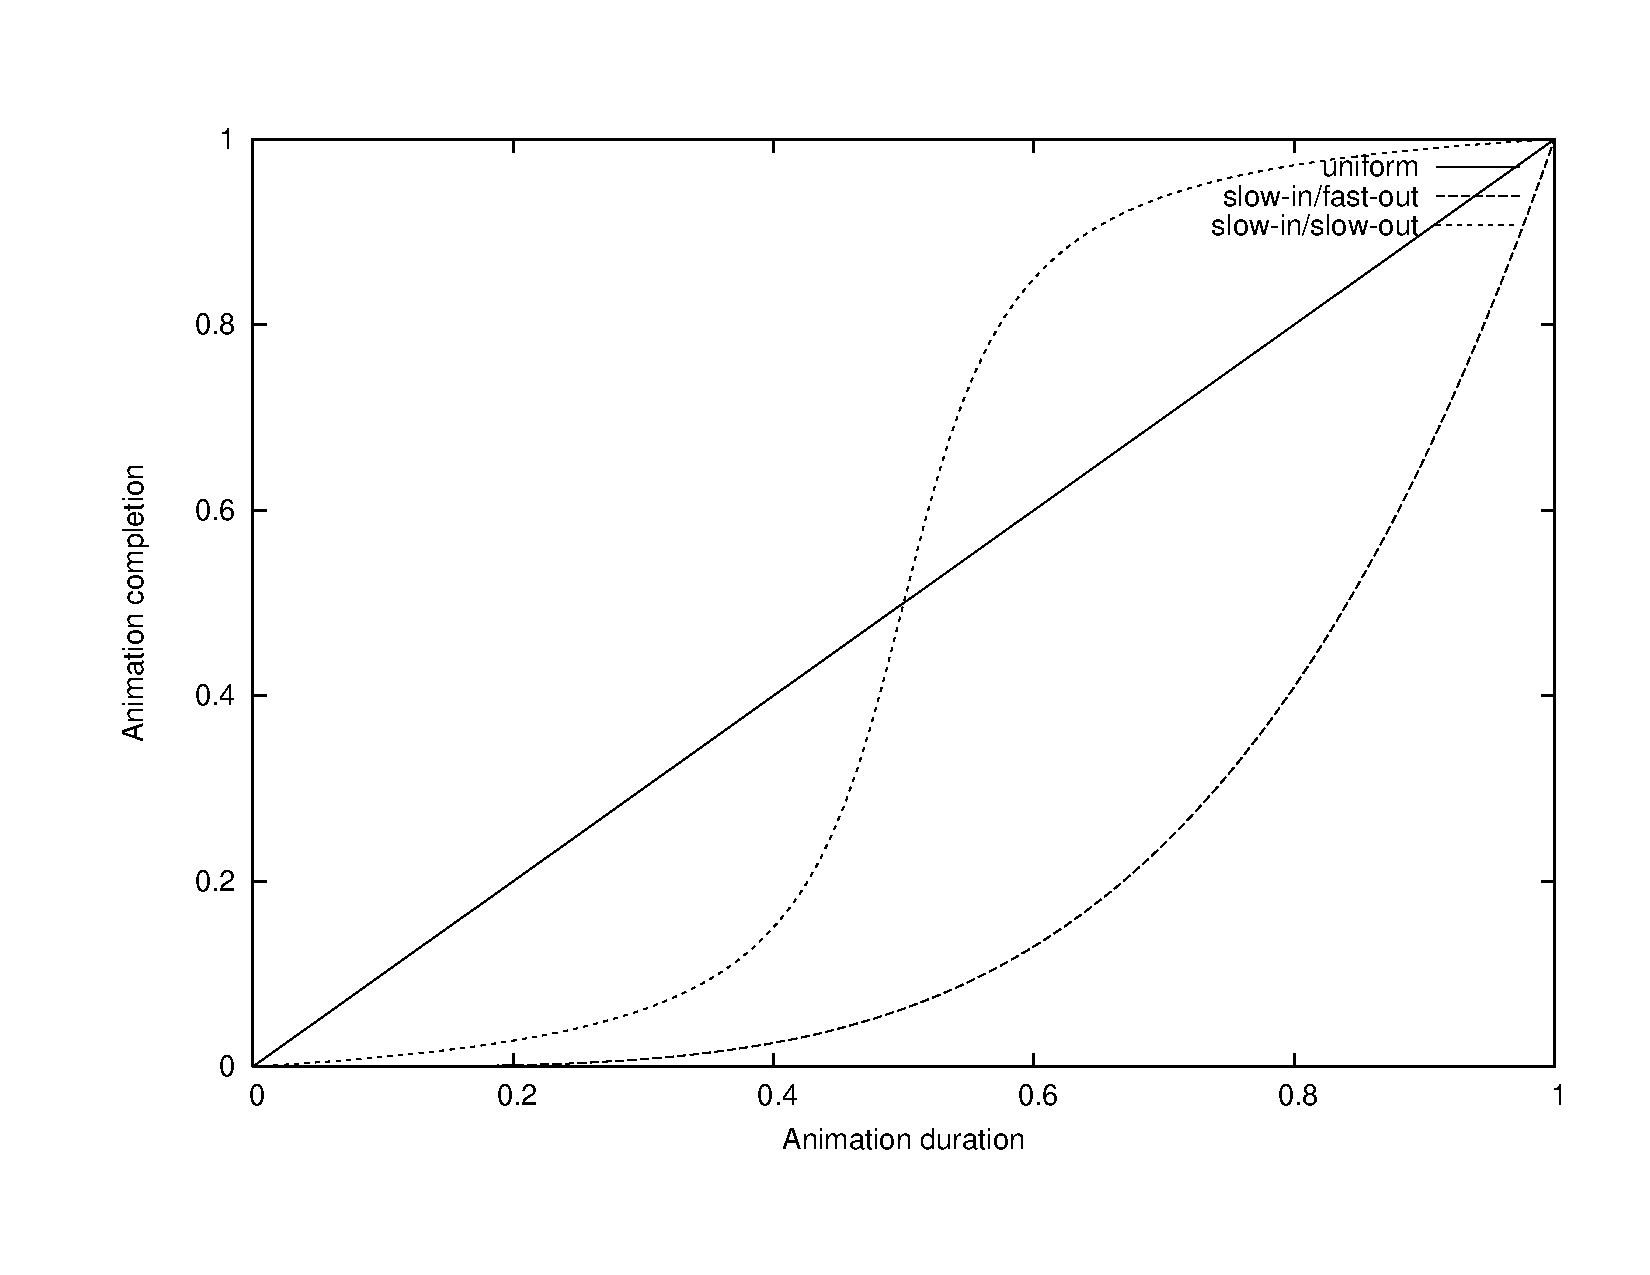
\includegraphics[width=16cm]{images/animSchem.pdf}
  \includegraphics[width=5.5cm,angle=-90]{images/animSchemEx.pdf}
   \caption{Animation pacing functions (top) and example on the translation of a rectangle (bottom)}
   \label{fig:pacing}
\end{figure}

Animations are specified with a single instruction and do not require much more code than the basic modification of a variable's value. They require the following parameters: the animation duration, the object involved, the variable(s) impacted by the animation, the desired target value, and the pacing function. Three off-the-shelf pacing functions are available (Figure \ref{fig:pacing}). Slow-in/slow-out transitions are typically used for camera motion and some glyph animations such as translations, as they convey a feeling of solidity that is important in direct manipulation interfaces \cite{Chang93}. Non-uniform pacing functions are generally used to put emphasis on the start (and/or end) of animation paths. However, they are not always appropriate, and the uniform function is often used when modifying, e.g., magnification lens parameters, or when animating color changes.

Animations are managed by a dedicated thread that controls their timing precisely, skipping steps on the computed animation path if necessary. This mechanism ensures that an animation lasts the specified duration, and runs as smoothly as the system and hardware performance allow. Until v0.9.8, ZVTM was using its own animation engine. Since v0.10.0, the animation engine has been completely rewritten and is now based on Sun's Timing Framework\fref{https://timingframework.dev.java.net/}, and now features additional capabilities in terms of animation management. The use of this more generic API should also make it easy for people already familiar with the Timing Framework to write animations in ZVTM. We only describe the new API in the following.

%%%%%%%%%%
\subsection{Animation Module: Overview}
The Animation module in ZVTM is heavily based upon the Timing Framework.

From this framework, we borrow the concepts of Timing Sources, Interpolators and Timing Targets 
(called Timing Handlers in our API). 
We discard the idea of an Animator targetting multiple receivers in favor of an Animation class
that animates a single object (Glyph, Camera, Portal, Lens or Translucent).
Sun's Timing Framework also provides animation triggers, which are not
replicated in our API.
\subsubsection{Animation}
The Animation class encapsulates an animation that has a single target and dimension.
Dimensions are enumerated in the \cd{Animation.Dimension} enum.

\subsubsection{AnimationManager}
The Animation manager is in charge of managing the queue system (more on that
below) and of controlling animations (conventional animations and the current camera 
animation). 

\subsubsection{AnimationFactory}
This class provides a number of Animation creation methods.

\subsubsection{TimingHandler Interface}
The TimingHandler interface defines a number of callbacks that custom animation developers
need to implement.
It looks like this:
\begin{small}
\begin{SaveVerbatim}{CodeVerb}
public interface TimingHandler {
    public void begin(Object subject, Animation.Dimension dim);

    public void end(Object subject, Animation.Dimension dim);

    public void repeat(Object subject, Animation.Dimension dim);

    public void timingEvent(float fraction, 
			    Object subject, Animation.Dimension dim);
}
\end{SaveVerbatim}
\fbox{\BUseVerbatim[boxwidth=0.99\columnwidth]{CodeVerb}}
\end{small}
\cd{begin} and \cd{end} are called once, respectively when the animation starts and ends. They are, of course, the ideal place for setup and teardown logic.
\cd{repeat} is called each time the animation loops.
\cd{timingEvent} is the "workhorse" method that implements most of the 
animation's behavior. It is called repetitively during the animation and provides the elapsed fraction of the animation, between 0 and 1.

%%%%%%%%%%
\subsection{Creating an Animation: the Flexible Way}
\label{sec:animflex}

The generic way to create an Animation is to use one of the three createAnimation() methods
of AnimationFactory. Here is an example:

\begin{small}
\begin{SaveVerbatim}{CodeVerb}
Animation cameraAlt =
  am.getAnimationManager().getAnimationFactory().createAnimation(
   4000, 
   2f,
   Animator.RepeatBehavior.REVERSE,
   vsm.getVirtualSpace("src").getCamera(0),
   Animation.Dimension.ALTITUDE,
   new DefaultTimingHandler(){
      public void timingEvent(float fraction, 
                              Object subject, 
                              Animation.Dimension dim){
         Camera c = (Camera)subject;
         c.setAltitude(25+Double.valueOf(fraction*50).doubleValue());
      }
                                             
      public void end(Object subject, Animation.Dimension dim){
         circle2.setColor(Color.RED);
      }
   },
   ConstantAccInterpolator.getInstance()
);
\end{SaveVerbatim}
\fbox{\BUseVerbatim[boxwidth=0.99\columnwidth]{CodeVerb}}
\end{small}

Creating an animation this way gives programmers freedom to implement 
any animation path, side-effect... in their TimingHandler-derived class.

For convenience, a \cd{DefaultTimingHandler} class is provided that overrides 
the \cd{begin}, \cd{end} and \cd{repeat} methods with empty stubs, leaving only the \cd{timingEvent} method to implement.

%%%%%%%%%%
\subsection{Creating an Animation: the Easy Way}
Ready-made Animation factory methods are provided to cover the most common
cases as part of the \cd{AnimationFactory} class. 
These factories are named create[TargetType][AnimationType].
For instance, a Glyph translation can be created by calling:

\codebox{vsm.getAnimationManager().getAnimationFactory().createGlyphTranslation(...);}

where \cd{vsm} is a reference to your application's \cd{VirtualSpaceManager}.

The target/type combinations provided are:
\begin{itemize}
  \item Camera altitude
  \item Camera translation
  \item Glyph border color
  \item Glyph fill color
  \item Glyph orientation
  \item Glyph size
  \item Glyph translation
  \item Lens magnification
  \item Lens radii
  \item Path animation
  \item Portal size
  \item Portal translation
  \item Translucency animation
\end{itemize}

An example of animation created in this way is:
\begin{small}
\begin{SaveVerbatim}{CodeVerb}
Animation anim = vsm.getAnimationManager().getAnimationFactory().createLensMagAnim(
         LENS_ANIM_TIME, (FixedSizeLens)lens, -2.0f, 
         true, IdentityInterpolator.getInstance(), 
         new EndAction(){
             public void execute(Object subject,
                 Animation.Dimension dimension){
                 vsm.getOwningView(((Lens)subject).getID()).setLens(null);
                 ((Lens)subject).dispose();
             }
        }); 
vsm.getAnimationManager().startAnimation(anim, true);
\end{SaveVerbatim}
\fbox{\BUseVerbatim[boxwidth=0.99\columnwidth]{CodeVerb}}
\end{small}

%%%%%%%%%%
\subsection{Controlling Animations}
Animations are controlled from the AnimationManager.
There is a unique animation manager per VirtualSpaceManager.
Once created, animations need to be explicitly started.
Animations will automatically stop after their programmed duration, but may
be stopped or cancelled early by the programmer.

\subsubsection{The Queue System}
Animations have a dimension property and a subject (the object being animated).
Two animations are said to conflict if they target the same subject \emph{and} have the same dimension.
Conflicting animations are executed in sequence, while orthogonal animations (those that do not conflict)
are executed concurrently.

The queue system can be thought of as a number of queues: one queue for each
(subject, dimension) pair, although it is not implemented in that way for efficiency reasons. 
Animations are put into those queues by calling AnimationManager.startAnimation().
The first animation of the queue is run, and will leave the queue upon completion 
when it will be replaced by the next animation in line, if any.

\subsubsection{Starting an Animation}
Given a reference \cd{anim} to an Animation that was created using the AnimationManager factory,
an Animation is started by calling

\codebox{am.startAnimation(anim, false)}

The boolean parameter will put \cd{anim} in the queue in the normal fashion if set to false,
or cancel all conflicting animations prior to enqueing \cd{anim} if set to true, thus
ensuring that the animation will start immediately. 
  
\subsubsection{Stopping or Cancelling an Animation}
Ending an Animation without waiting for completion is done through the
AnimationManager's \cd{stopAnimation} and \cd{cancelAnimation} methods.
Both take a single parameter: a reference to the \cd{Animation} that must be stopped or cancelled.
The difference between stopping and cancelling an Animation is that the end action (\cd{end} method
of a \cd{TimingHandler} or \cd{execute} method of an \cd{EndAction} will be executed if the animation
is stopped, but not if it is cancelled.

\subsubsection{Pausing and Resuming an Animation}
In addition to starting, stopping and cancelling Animations, it is possible to put them on hold.
The relevant AnimationManager methods are \cd{pauseAnimation} and \cd{resumeAnimation}, 
both of which take the animation to pause or resume as their only parameter, and return a boolean
indicating whether the animation was successfully paused or resumed.

%%%%%%%%%%
\subsection{Current Camera Animation}  
Parallel to the animation mechanism described above, the AnimationManager has a 
built-in mechanism to animate the current Camera in an interactive fashion. This is
typically used to implement rate-based scrolling and zooming.

To directly animate the current Camera, set its X, Y, and Z speeds using the corresponding AnimationManager
methods \cd{setXspeed}, \cd{setYspeed} and \cd{setZspeed}.
The X, Y, and Z speed units are arbitrary, but the X and Y speed units are consistent
(if the X speed and Y speed are equal, the camera will move at the same rate 
and in the same direction along the X and Y axes).

Examples of rate-based scrolling using the current camera animation are found in several places 
throughout the code, for instance every Animation example (in 
package \cd{fr.inria.zvtm.animation.examples}) implements it.

The current camera animation never conflicts with animations in the queue system
(i.e. it will run concurrently with any animation in the queue system).

%%%%%%%%%%
\subsection{Example of Custom Glyph Variable Animation}

Ready-made animation factory methods only cover the generic visual variables that apply to all types of glyphs. To animate visual variables defined only for some specific type of glyph, one can use the \cd{createAnimation()} methods of \cd{AnimationFactory}. The following example shows how to animate a \cd{VRing} so that it behaves like a circular progress indicator:
\begin{small}
\begin{SaveVerbatim}{CodeVerb}
Animation anim = 
    vsm.getAnimationManager().getAnimationFactory().createAnimation(
        timeout, glyphs[0], Dimension.PATH, new DefaultTimingHandler() {
          @Override
          public void timingEvent(float fraction, Object target, Dimension dim) {
              ((VRing)target).setAngle(fraction * 2*Math.PI);
              ((VRing)target).orientTo(fraction * Math.PI + Math.PI / 2);
          }

          @Override
          public void begin(Object subject, Dimension dim) {
              super.begin(subject, dim);
              ((VRing) subject).setAngle(0);
          }
    });

    vsm.getAnimationManager().startAnimation(anim, false);
\end{SaveVerbatim}
\fbox{\BUseVerbatim[boxwidth=0.99\columnwidth]{CodeVerb}}
\end{small}



